\documentclass[letterpaper, 10 pt, conference]{ieeeconf}  % Comment this line out if you need a4paper
%\documentclass[a4paper, 10pt, conference]{ieeeconf}      % Use this line for a4 paper
\IEEEoverridecommandlockouts        
\overrideIEEEmargins                  
%\pdfobjcompresslevel=0
%\pdfminorversion=4
\usepackage{graphics} % for pdf, bitmapped graphics files
\usepackage{epsfig} % for postscript graphics files
\usepackage{mathptmx} % assumes new font selection scheme installed
\usepackage{times} % assumes new font selection scheme installed
\usepackage{amsmath} % assumes amsmath package installed
\usepackage{amssymb}  % assumes amsmath package installed
\usepackage{footnote}
\makesavenoteenv{tabular}
\makesavenoteenv{table}
\usepackage{multicol}
\usepackage{cite}
\usepackage{tabu}
\usepackage{hyperref} 
\usepackage{amsmath,amssymb,amsfonts}
\usepackage{algorithmic}
\usepackage{graphicx}
\usepackage{textcomp}
\usepackage{xcolor}
\usepackage[utf8]{inputenc}
\usepackage[english]{babel}
\usepackage{amstext}
\usepackage{subcaption}
\usepackage[utf8]{inputenc}
\usepackage[export]{adjustbox}
\usepackage{wrapfig}
\usepackage{hyperref}% if you want/for demonstration of  hyperlinks
\usepackage{footnotebackref}
\usepackage{footnote}
\usepackage{rotating}
\usepackage{tablefootnote}
\usepackage{float}
\usepackage{placeins}
\usepackage{ragged2e}
\usepackage{latexsym}
\usepackage{amsfonts}
\usepackage{amssymb}
\usepackage{booktabs}
\usepackage{tabularx}
\usepackage{float}
\usepackage{etoolbox}
\usepackage{tikz}
\usepackage{graphicx}
\usetikzlibrary{positioning}

\title{\LARGE \bf
Perception of Social Intelligence in Robots Performing False-Belief Tasks
}

\author{Stephanie Sturgeon, Andrew Palmer, Janelle Blankenburg, and David Feil-Seifer \\
Department of Computer Science \& Engineering \\
University of Nevada, Reno\\ Reno, NV 89557 \\
stephaniesturgeon@gmail.com, ahpalmer@nevada.unr.edu, jjblankenburg@nevada.unr.edu,
dave@cse.unr.edu
} 


\begin{document}
\maketitle
%\thispagestyle{empty}
%\pagestyle{empty}
%%%%%%%%%%%%%%%%%%%%%%%%%%%%%%%%%%%%%%%%%%%%%%%%%%%%%%%%%%%%%%%%%%%%%%%%%%%%%%%%
\begin{abstract}
This study evaluated how a robot demonstrating a Theory of Mind (ToM) influenced human perception of social intelligence and animacy in a  human-robot interaction. Data was gathered through an online survey where participants watched a video depicting a NAO robot either failing or passing the Sally-Anne false-belief task. Participants (N = 60) were randomly assigned to either the Pass or Fail condition. A Perceived Social Intelligence Survey and the Perceived Intelligence and Animacy subsections of the Godspeed Questionnaire Series (GQS) were used as measures. The GQS was given before viewing the task to measure participant expectations, and again after to test changes in opinion. Our findings show that robots demonstrating ToM significantly increase perceived social intelligence, while robots demonstrating ToM deficiencies are perceived as less socially intelligent. 
\end{abstract}
%%%%%%%%%%%%%%%%%%%%%%%%%%%%%%%%%%%%%%%%%%%%%%%%%%%%%%%%%%%%%%%%%%%%%%%%%%%%%%%%
\section{Introduction}
Computers, virtual assistants, and robots are becoming increasingly accessible, and as a result these systems are commonly integrated into our personal and professional routines. The more we interact with these systems it appears that humans are able to anthropomorphize these non-human entities when they exhibit aspects of social cognition \cite{VANDERWOERDT201993}\cite{Reeves}. Social-cognitive processes are essential not just for human-human teamwork, but also for human-robot teamwork. By advancing social capabilities for robots, interactions with humans can become more natural\cite{BREAZEAL2002481}. Social intelligence is essential to creating smarter and behaviorally human-like robots \cite{Dautenhahn94, dautenhahn98, dautenhahn2004}. Theory of Mind (ToM) is the ability to infer the thoughts, feelings, and beliefs of others \cite{BARONCOHEN85}. The capacity for Theory of Mind marks a fundamental precursor to other social cognitive development in humans, and is therefore the focus of this study. Being able to distinguish `self' from `other' is fundamental in social interactions and interpreting social cues.

How socially intelligent we perceive a machine or even other humans to be determines what we expect them to understand and affects how we interact with them. When automated telephone systems or chat bots violate social cues or it becomes clear the  needs of the human aren't understood, then perception of agency declines and the interaction becomes strained\cite{Wallis, IJoC6277}. Similarly, when a robot violates social distance norms, that lack of consideration for other people can be perceived as a lack of intelligence~\cite{forer2018socially-aware, feil-seifer2012distance-based}.

The ability to read social cues could dramatically improve the effectiveness of socially assistive systems. Research shows that displaying human-like learning behavior increases perceived intelligence of robots as well as satisfaction with human-robot interaction \cite{Rosenthal-von}. Another study showed using social cues such as mimicry increased perceived intelligence of artificial agents which has been suggested to increase compliance during interaction with artificial systems\cite{Kaptein}. Intuitively, it makes sense that participants would rate a robot favorably who demonstrates a human-like cognitive process such as Theory of Mind. 

In this paper, we present an experiment that studies the effect of observed deficiencies in ToM behavior on perceived social intelligence. This will serve to both establish the baseline expectation that people observing a robot have regarding ToM as well as the effect that supporting/confounding that belief will have on perceived social intelligence.


%%%%%%%%%%%%%%%%%%%%%%%%%%%%%%%%%%%%%%%%%%%%%%%%%%%%%%%%%%%%%%%%%%%%%%%%%%%%%%%%

\section{Background}
 In this section, we discuss related work which provides background for the cognitive process focused on in this study, how it can potentially play a role in Human-Robot Interaction, and how we arrived at our hypotheses.
 %We also discuss the questionnaires we will be drawing from for our pre-task and post-task survey.
 
%\subsection{Perception in HRI}
%Research in the field of Human-Robot Interaction shows robots with social capabilities are more readily accepted by humans, communicate more efficiently, and are interpreted as being more enjoyable and useful to interact with \cite{BREAZEAL2003119},\cite{Heerink2010}, \cite{shin}.

\subsection{Theory of Mind}
Theory of Mind (ToM) or mentalizing refers to the ability to make inferences about the thoughts, beliefs, or intentions of another individual \cite{BARONCOHEN85}. ToM is what facilitates the ability to make inferences about the mental states of others from their actions. Being able to infer the intentions of others is critical in communication and social interactions. The ability to anticipate and relate to human intentions will create more natural social interactions between humans and robots as well as impact how socially and emotionally intelligent we perceive them.

Theory of Mind deficits in adults are associated with conditions such as Autism Spectrum Disorder (ASD)\cite{ASD1},\cite{ASD2},\cite{ASD3}, frontal variant frontotemporal dementia \cite{10.1093/brain/awf079, TORRALVA2007342}, and Schizophrenia \cite{Schizophrenia},\cite{Schizophrenia2}. Such deficits result in difficulty reading social cues and perceptions, and this is usually interpreted as deviant behavior. One mock trial study told half of the participants that the defendant had ASD and were given information about the condition, while the other half were not given any of this info, and they found that participants without defendant background scored him as less likable, less honest, assigned higher blame and guilt, as well as perceiving him to be rude, aggressive, and having no remorse \cite{Maras2019}. Theory of Mind is a critical component in social norms and influences our perception of both humans and robots who have these deficits. 

\subsection{False Belief}
%The Sally-Anne false belief task and narrative variations of it are the standard test for Theory of Mind. This is typically used with children between four to six years old to see if they have developed the ability to distinguish the difference between what they know and diverging information in others.

One of the earliest tests for Theory of Mind developed by Baron-Cohen et al. is the Sally-Anne false belief task \cite{BARONCOHEN85}. The classic version is either shown as a cartoon or acted out with dolls. Children are shown two girls, one named Sally who puts a ball into a basket and then goes for a walk. The other girl, Anne, takes the ball from the basket and places it in a box. When Sally returns the child is asked where she will look for the ball. To pass the task, the child needs to answer correctly that Sally \textit{believes} the ball to still be in the basket. If the child answers the belief question from their own perspective then they fail to see that Sally has her own thoughts and beliefs about reality.

The task in this study is a variation of the Sally-Anne false-belief task in which we act out the scenario in front of a robot instead of a child. The robot is then asked the standard Sally-Anne task questions about the ball's current and previous locations as well as where Sally (Experimenter A in our scenario) believes the ball to be. The task in this study is staged. We are primarily focused on the reactions to the task, therefore we did not attempt to implement autonomous functionality for our robot, but rather relied on pre-scripted interaction. Our robot will answer the belief question incorrectly in the \textbf{Fail} condition, and will answer correctly in the \textbf{Pass} condition.

\subsection{Theory of Mind and Robotics}

%%% need to fill in %%%

Early robotics research has promoted ToM capability for humanoid robots. This early work has centered on faces and animate stimuli~\cite{scassellati2002theory}. This then led to robotic self-recognition through probabilistic reasoning over visual information~\cite{gold2009using}. Later work made an autonomous robot system that can estimate the mental states of other agents~\cite{devin2016implemented}. Such interpretation can be utilized to distinguish between multiple related plans based on the robot's belief of their human partner's intentions~\cite{hiatt2011accommodating}. Thus, robotics that employ ToM capability can possibly better understand and interpret human behavior by creating a mental model of human attention~\cite{kramer2011theory}. However, none of this work directly addresses how a human interacting with a robot that utilizes such a mental model might change its interpretation of the robots' capabilities.

%There have been a few proposals for how to implement ToM abilities in robots in order to facilitate more natural interactions and human-like social learning through observation \cite{Scassellati}, \cite{Devin}. Robots who are able to make inferences about human mental states and intentions would be..
%%% Stephanie %%%




%%%%%%%%%%%%%%%%%%%%%%%%%%%%%%%%%%%%%%%%%%%%%%%%%%%%%%%%%%%%%%%%%%%%%%%%%%%%%%%%
\section{Methodology} 

\begin{figure}[t]
\begin{center}
\begin{subfigure}{0.98\linewidth}
\centering
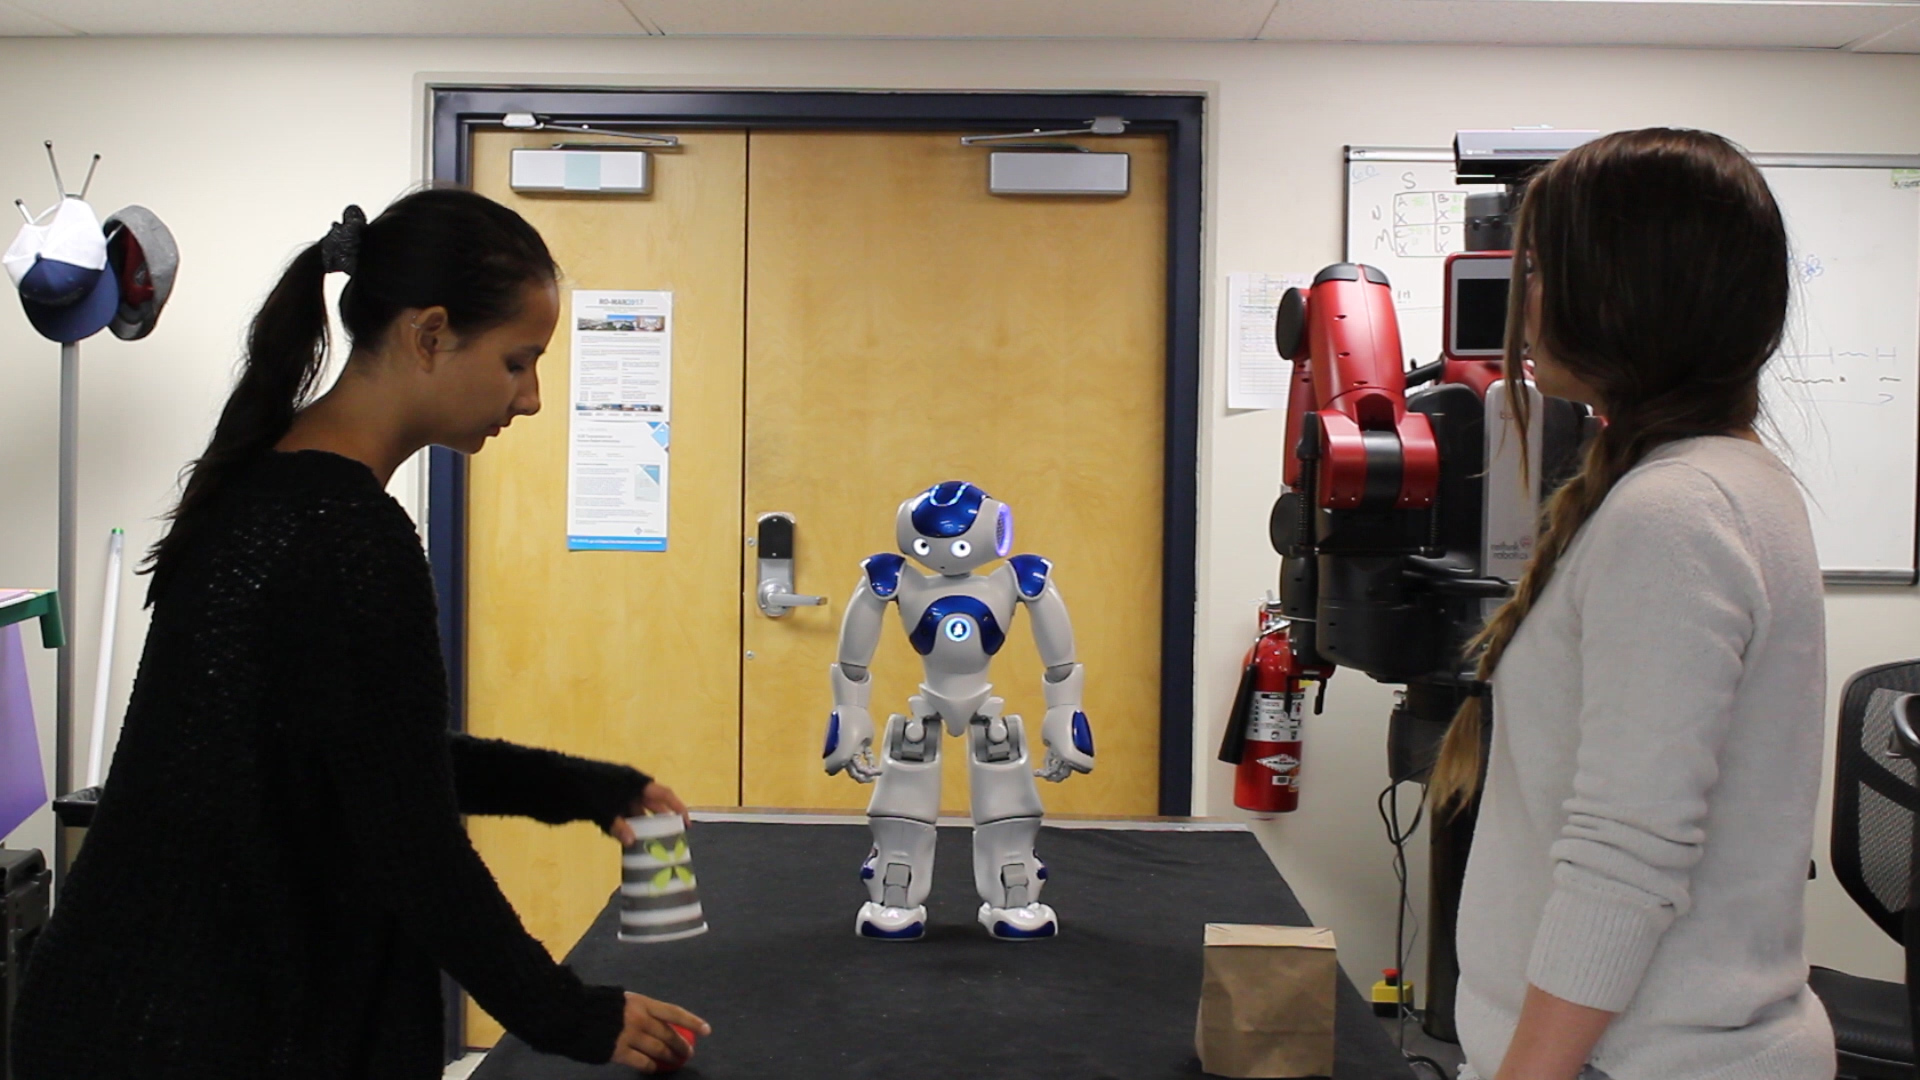
\includegraphics[width=0.9\linewidth]{cup.jpg}
\caption{Experimenter A (Sally) places the ball under the cup before leaving the room\label{fig:Task1}\vspace{0.3cm}}
\end{subfigure}
\begin{subfigure}{0.98\linewidth}
\centering
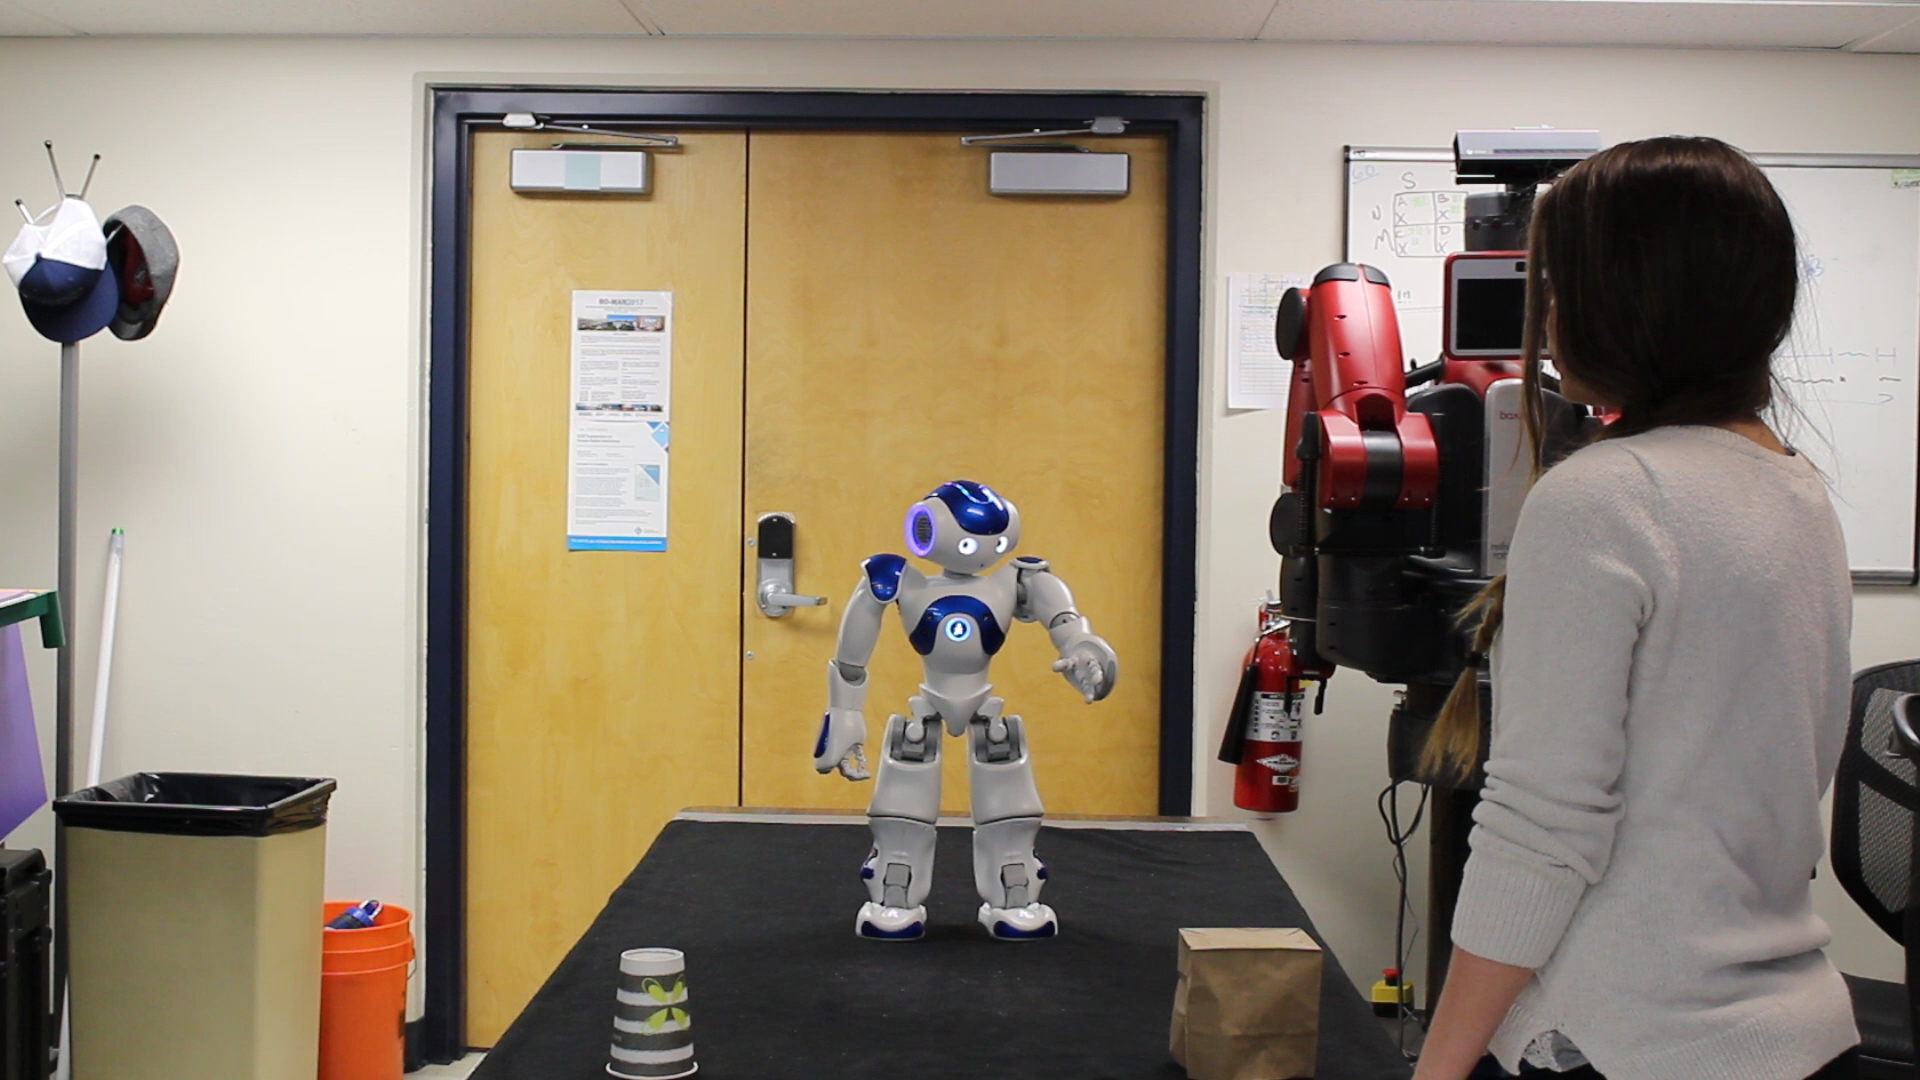
\includegraphics[width=0.9\linewidth]{where_is_it.jpg} 
\caption{``Where is the ball right now?"}
\label{fig:Task2}\vspace{0.3cm}
\end{subfigure}
\begin{subfigure}{0.98\linewidth}
\centering
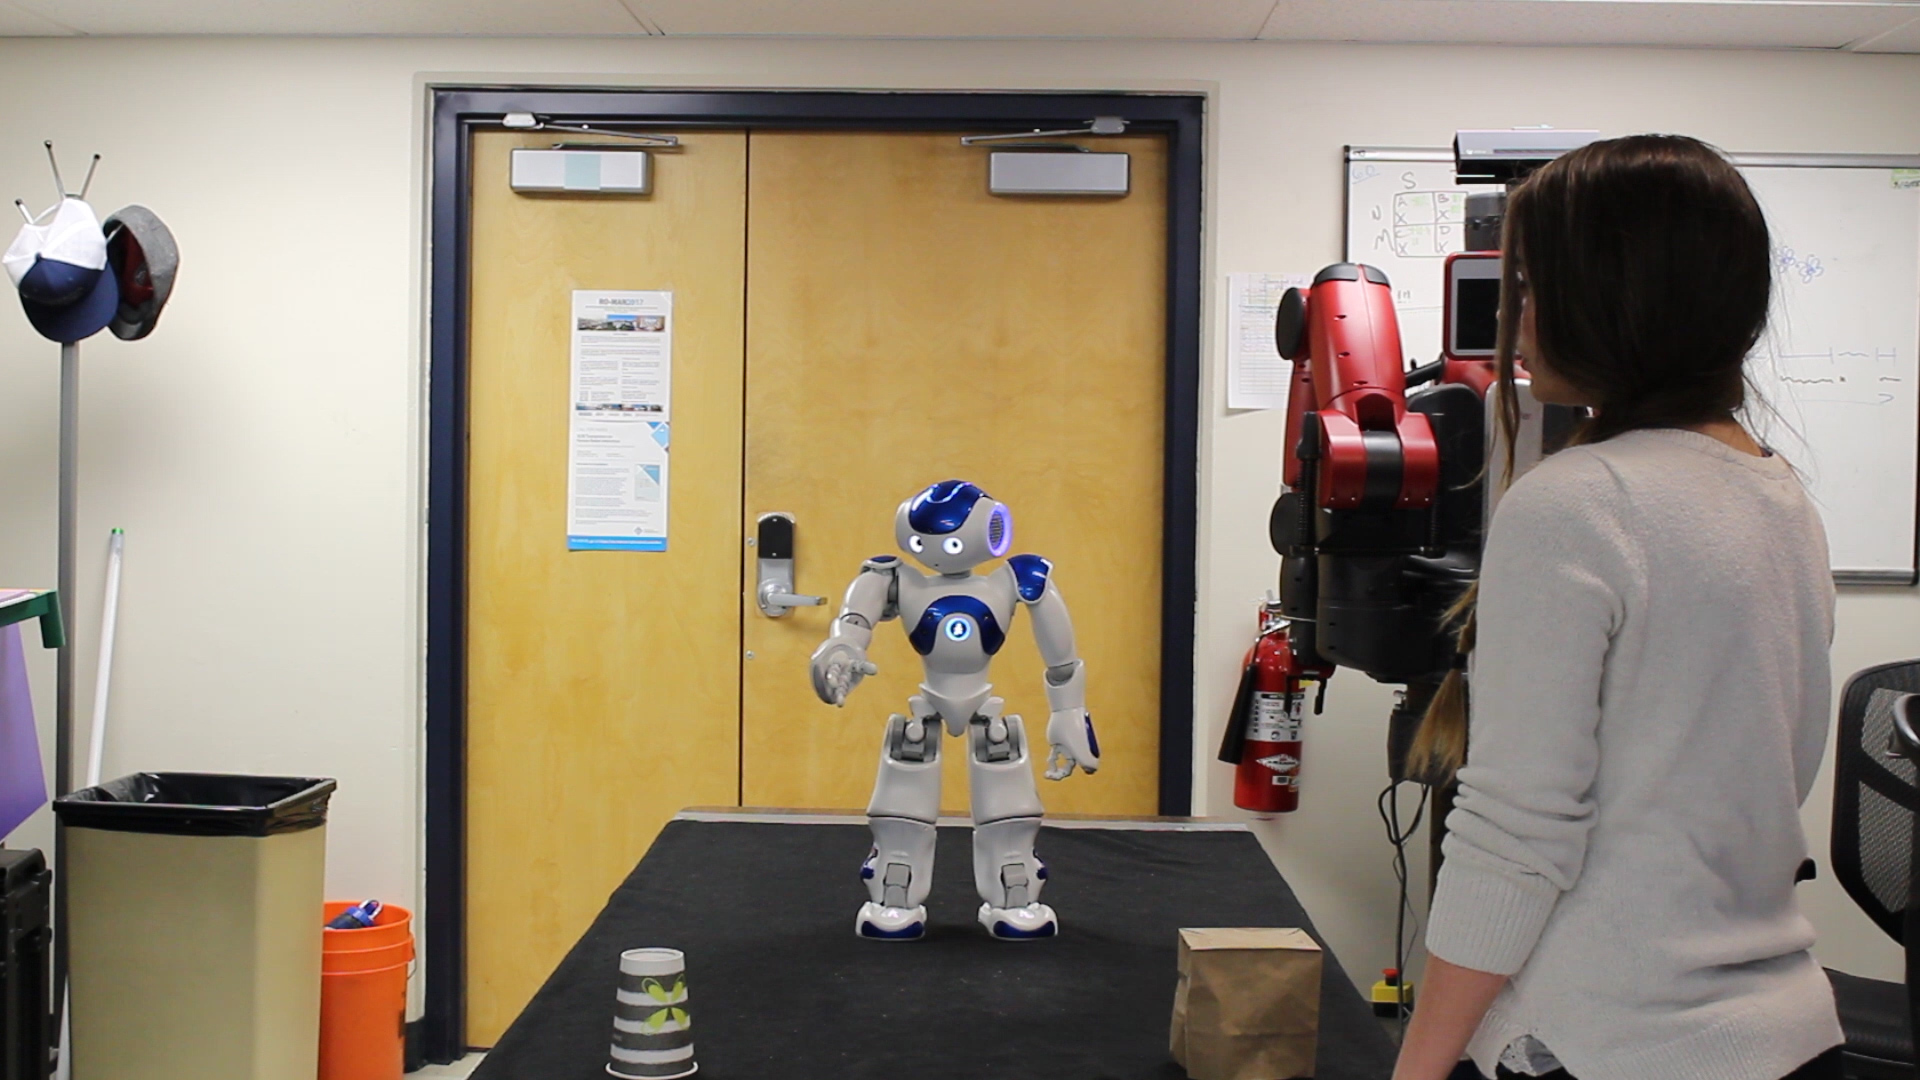
\includegraphics[width=0.9\linewidth]{where_was_it.jpg}
\caption{``Where was the ball when she left the room?"}
\label{fig:Task3}
\end{subfigure}
\end{center}
\caption{Experiment setup - All participants regardless of condition watch this sequence}
\label{fig:image2}
\end{figure}


%%% Study purpose %%%
We examine ToM in this study in order to see how an anthropomorphic robot demonstrating human-like cognitive reason such as belief tracking would be interpreted. Additionally, we intended to validate the Perceived Social Intelligence Survey \cite{PSI}. 

\subsection{Experiment Design}

Participants watched a NAO robot perform a variation of the Sally-Anne false belief task. The participants were asked to observe a video of a robot as it oversees a simple task. Experimenter A (in view of the robot) places a ball under a cup. That experimenter then leaves the room. When A is out of the room, a false belief can be created if Experimenter B then moves the ball from under the cup to under the bag (in view of the robot, but not experimenter A). The task setup is shown in Figure~\ref{fig:image2}.

Participants watched experimenter A (Figure~\ref{fig:Task1}, left) place a ball under the cup and then leave the room. Experimenter B (Figure~\ref{fig:Task2}, right) then moves the ball under the bag (in view of the robot), however, experimenter A did not see this move and should still believe that the ball is under the cup. The robot is then asked about the ball's current and previous location (Figure~\ref{fig:Task3}).

The video stops and the participant was asked a question meant to determine if they believed that the robot has the capacity for Theory of Mind. Participants were asked where the robot thinks the experimenter A will now look for the ball. The participant is then played a video showing experimenter A walking back into room, and the robot is asked where Experimenter A will look for the ball. The response varies depending on participant condition. Those in the {\bf Pass} condition saw the robot look, point, and say `She will look under the cup' and those in the {\bf Fail} condition saw the robot look, point, and say `She will look under the bag.' 


\subsection{Experimental Hypotheses}

Based on existing literature in human-robot interaction and cognitive science we propose four hypotheses to be explored in this study: \newline
\textbf{H1:}The robot that demonstrates ToM behavior will be perceived as more socially intelligent than one that does not.\newline
\textbf{H2:}The robot that demonstrates ToM behavior will be perceived as more animate than one that does not.\newline
\textbf{H3:}An observer's perception of the robot's social intelligence will be greater after observing ToM behavior than before observing any social behavior.\newline
\textbf{H4:}A participant would expect the robot to be able to demonstrate ToM behavior.
 
\subsection{Participants}

An online survey was created using the Qualtrics Research Core platform \cite{Qualtrics} to show either the {\bf Pass} or {\bf Fail} condition. Participants ($n = 60$, $60\%$ male) were asked to watch a video and complete an online survey. Most ($n = 53$) participants were college educated from `some college' up to a `PhD', and seven participants had only a high school diploma. The age range of the participants was between $20-79$ years old. Career field was given two categories: professional, scientific, and information technology ($n= 28$), and other ($n=32$). Recruitment was done through word of mouth and social media (Facebook and Instagram).  

\subsection{Measures}
Five demographic questions were asked to see if there were any correlations between career industry, age, gender, education level, or previous experience with robots. We administered the Godspeed Questionnaire Series (GQS) \cite{BARTNECK} and the Perceived Social Intelligence Survey (PSI) \cite{PSI}. The GQS uses a 5-point bipolar scale and the PSI utilizes multiple 5-point likert scale questions for each inventory item.

From the GQS, the perceived intelligence and animacy scales were chosen in order to see the impact of an anthropomorphic robot such as the NAO demonstrating ToM on how people would perceive life-likeness and intelligence. These scales were administered both before and after viewing the task. This allowed us to observe any change in opinion after ToM capability is demonstrated/not demonstrated.  GQS-Perceived Intelligence and GQS-Animacy scale were used to examine \textbf{H1} and \textbf{H2}.

During the video, three questions are asked: {\em Where is the ball, currently?}, {\em Where was the ball when experimenter A left the room?} and, {\em Where will experimenter A look for the ball?} We stopped the video before the last question to ask participants how they expect the robot to answer. The options were under the cup or under the bag. We did this to test \textbf{H4} and see whether participants already had an expectation for the robot to possess this ToM behavior.

Following the video presentations, the participants were then given the Perceived Social Intelligence (PSI) questions. The scales used from the PSI Survey are as follows: Recognizes Human Behavior (RB), Recognizes Human Cognition (RC), Adapts to Human Behavior (AB), Adapts to Human Cognitions (AC), Predicts Human Behavior (PB), Predicts Human Cognitions (PC), Identifies Individuals (II), and Socially Competent (SOC). These scales detect social information processing abilities. The scales RC, AC, and PC were of particular interest for both \textbf{H1} and \textbf{H3} as they directly relate to definitions for ToM. The scales RB, AB, and II were selected because they relate to precursors to ToM \cite{scassellati2002theory}. Lastly, we wanted to see how overall social competence would be perceived after viewing the task.


%%%%%%%%%%%%%%%%%%%%%%%%%%%%%%%%%%%%%%%%%%%%%%%%%%%%%%%%%%%%%%%%%%%%%%%%%%%%%%%%
\section{Results}
Z-scores were calculated for individual items for both the Godspeed Questionnaire and Perceived Social Intelligence Survey. For statistical tests which require continuous dependent variables, composite Z-score were used. This section reports scales with statistical significance.

\subsection{Internal Consistency}
The GQS questionnaire was employed to measure different, underlying constructs. One construct, `Perceived Intelligence', consisted of five questions. The scale had internal consistency, as determined by a pre-task Cronbach's $\alpha = 0.758$ as well as post-task $\alpha = 0.881$. One construct, 'Animacy', consisted of 6 items. The scale had an  $\alpha = 0.646$ pre-task and $\alpha = 0.770$ post-task.

The PSI scales were also tested for reliability. All scales consisted of four questions. The following scales all had internal consistency, as determined by Cronbach's alpha: PSI-AB ($\alpha = 0.779 $), PSI-AC ($\alpha = 0.743$), PSI-RC ($\alpha = 0.769$), PSI-PC ($\alpha = 0.797$), PSI-II ($\alpha = 0.832$), and PSI-SC ($\alpha = 0.770$).  PSI-PB ($\alpha = 0.680$) and PSI-RB $\alpha = 0.418$ had lower levels of internal consistency than any of the other PSI scales.

\subsection{Godspeed Questionnaire Series}
From the GQS there was only statistical significance found for the Perceived Intelligence scale. Mann-Whitney U Tests were conducted to determine if there were differences in the Perceived Intelligence post-task scores as well as the difference scores between the Pass and Fail conditions. Distributions between the Pass and Fail conditions for both Perceived Intelligence post-task scores and the difference scores were not similar. Perceived Intelligence post-task scores for the Pass condition (mean rank = 37.21) were significantly higher than the Fail condition (mean rank = 24.63), U = 260.0, p $<$ 0.01. Similarly, Perceived Intelligence difference scores for Pass condition (mean rank = 36.02) were significantly higher than the Fail condition (mean rank = 25.67), U = 293.5, p $<$ 0.05.
\begin{table}[h!]
\centering
\caption{Godspeed Questionnaire Series Items}
\begin{tabular}{| c c |}
\hline
\textbf{Survey Questions} &  \textbf{Scale} \\ \hline
Incompetent / Competent &Perceived Intelligence\\
Ignorant / Knowledgeable &Perceived Intelligence\\
Irresponsible / Responsible &Perceived Intelligence\\
Unintelligent / Intelligent &Perceived Intelligence\\
Foolish / Sensible  &Perceived Intelligence\\
Dead / Alive &  Animacy \\
Stagnant / Lively  &Animacy \\
Mechanical / Organic &Animacy \\
Artificial / Lifelike &Animacy \\
Inert / Interactive &Animacy \\
Apathetic / Responsive &Animacy \\
\hline
\end{tabular}
\end{table}

\subsection{Perception of Intelligence When Expectations Were Met}
We used a Mann-Whitney U test to determine if there were differences in Perceived Intelligence scores between conditions when they answered the mid-task question expecting the robot to pass (N = 46). Distributions of the Perceived Intelligence scores for the Pass and Fail conditions were not similar. Perceived intelligence scores for the Pass condition (mean rank = 28.93) were statistically significantly higher than for the Fail condition (mean rank = 18.07), U = 389.5, Z = 2.751, p $<$ 0.01.

\begin{figure}
\centering
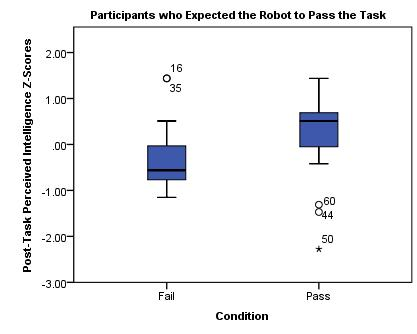
\includegraphics[ height=5cm]{Expectation-boxplot.jpg}
\caption{Perceived Intelligence scores were significantly higher in the Pass condition (p $<$ 0.01) when their expectations for the robot were met supporting H3.}\label{fig:expectation-boxplot}
\end{figure}

\subsection{Perceived Social Intelligence Scales}

Analysis of the composite scores for the PSI found statistically significant results for the following scales: RC, PC, AC, PB, II, and SOC.

\subsubsection{Recognizes Human Cognitions (RC)}

A Kruskal-Wallis test was used to determine if there were differences in RC scores between participants that watched the robot either pass or fail the false belief task. Distributions of RC scores were not similar for all groups, as assessed by visual inspection of a boxplot. RC scores were significantly different between conditions, \begin{math}\chi ^2= 20.508, p < 0.001 \end{math}. The Fail group had a mean rank = 20.95 and the pass group had a mean rank = 41.41. 

\begin{figure}[h]
\centering
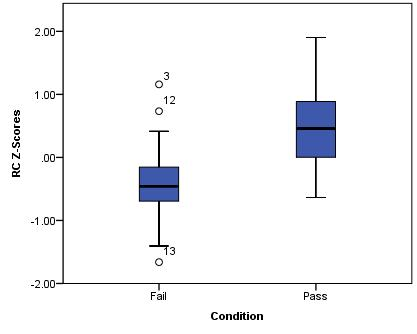
\includegraphics[ height=5cm]{RC.jpg}
\caption{RC Scores were significantly higher in the Pass condition $(p < 0.001)$ supporting H1.}
\label{fig:RC}
\end{figure}


\begin{table}[h]
\caption{Recognizes Human Cognition (RC) Items}
\begin{center}
\begin{tabu}{|p{1.5cm} p{6cm}|}
\hline
\textbf{Survey Questions} &(On a scale of Strongly Disagree to Strongly Agree)\\
\hline
This robot: &
\begin{itemize}
\item Can figure out what people think
\item Knows when people are missing information
\item Can figure out what people can see
\item  Understands others' perspectives
\end{itemize}\\
\hline
\end{tabu}
\label{RC}
\end{center}
\end{table}

\subsubsection{Predicts Human Cognitions (PC)}

A one-way ANOVA was conducted to determine if the perception of a robot being able to predict the cognition of humans was different depending on condition. There were no outliers for condition, as assessed by boxplot; data was normally distributed for each group, as assessed by Shapiro-Wilk test ($p > 0.05$); and there was homogeneity of variance, as assessed by Levene's test of homogeneity of variance for Condition (p = 0.706). The differences between conditions were statistically significant with the Pass condition (M = 0.352, SD = 0.760) being higher than the Fail condition (M = -0.308, SD = 0.686), F(1,58)= 12.498, p = 0.001. 

\begin{figure}[h]
\centering
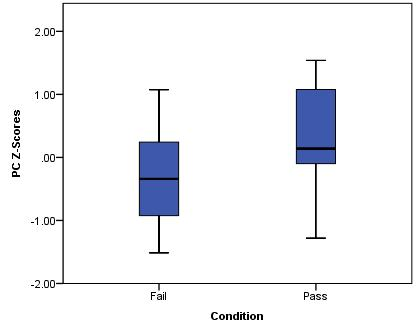
\includegraphics[ height=5cm]{PC.jpg}
\caption{PC scores in the Pass condition were significantly higher than the Fail condition (p $<$ 0.001) supporting H1.}
\label{fig:PC}
\end{figure}

\begin{table}[h]
\caption{Predicts Human Cognition (PC) Items}
\begin{center}
\begin{tabu}{|p{1.5cm} p{6.5cm}|}
\hline
\textbf{Survey Questions} &(On a scale of Strongly Disagree to Strongly Agree)\\
\hline
This robot: &
\begin{itemize}
\item Anticipates others' beliefs
\item Figures out what people will believe in the future
\item Knows ahead of time what people will think about certain situations 
\item Anticipates what people will think
\end{itemize}\\
\hline
\end{tabu}
\label{PC}
\end{center}
\end{table}

\subsubsection{Adapts to Human Cognitions (AC)}

A one-way ANOVA was conducted to determine if the perception of a robot being able to adapt its own behavior based on people's thoughts and beliefs was different depending on condition. There were no outliers, as assessed by boxplot; data were normally distributed for each condition, as assessed by Shapiro-Wilk test $(p > 0.05)$ and there was homogeneity of variance, as assessed by Levene's test of homogeneity of variance (p = 0.333). The Pass condition gave significantly higher AC scores (M = 0.245, SD = 0.635) than the Fail condition (M = -0.2147, SD = 0.789), F(1,58) = 6.075, p $<$ 0.05. 

\begin{figure}[H] 
\centering
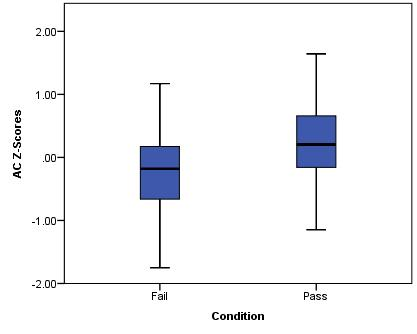
\includegraphics[ height=5cm]{AC.jpg}
\caption{AC scores were significantly higher (p $<$ 0.05) when ToM behavior was demonstrated supporting H1.}\label{fig:AC}
\end{figure}

\begin{table}[H]
\caption{Adapts to Human Cognition (AC) Items}
\begin{center}
\begin{tabu}{|p{1.4cm} p{6cm}|}
\hline
\textbf{Survey Questions} &(On a scale of Strongly Disagree to Strongly Agree)\\
\hline
This robot: &
\begin{itemize}
\item  Adapts its behavior based upon what people around it know
\item Ignores what people are thinking
\item Selects appropriate actions once it knows what others think
\item Knows what to do when people are confused
\end{itemize}\\
\hline
\end{tabu}
\label{AC}
\end{center}
\end{table}

\subsubsection{Predicts Human Behavior (PB)}
A Kruskal-Wallis test was conducted to determine if there were differences in PB scores between conditions. Distributions of PB scores were not similar for all conditions, as assessed by visual inspection of a boxplot. PB scores were statistically significantly different between conditions,  \begin{math}\chi ^2 = 4.462, p < 0.05 \end{math}. The Fail Condition had a mean rank = 26.05 and the Pass Condition had a mean rank = 35.59. 

\begin{figure}[h]
\centering
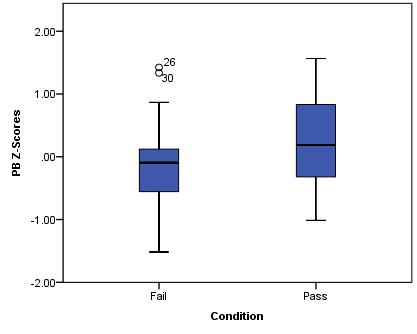
\includegraphics[ height=5cm]{PB.jpg}
\caption{PB Scores were significantly higher for the Pass condition (p $<$ 0.05) supporting H1.}
\label{fig:PB}
\end{figure}

\begin{table}[h]
\caption{Predicts Human Behavior (PB) Items}
\begin{center}
\begin{tabu}{|p{1.5cm} p{6cm}|}
\hline
\textbf{Survey Questions} &(On a scale of Strongly Disagree to Strongly Agree)\\
\hline
This robot: &
\begin{itemize}
\item  Anticipates people's behavior
\item Predicts human movements accurately
\item Has no idea what people are going to do
\item Knows how people will react to things it does
\end{itemize}\\
\hline
\end{tabu}
\label{PB}
\end{center}
\end{table}

\subsubsection{Identifies Individuals (II)}
A one-way ANOVA was conducted to determine if II scores were different depending on condition. There were no outliers for condition, as assessed by boxplot; data was normally distributed for each condition, as assessed by Shapiro-Wilk test ($p > 0.05$); and there was homogeneity of variance, as assessed by Levene's test of homogeneity of variance for condition (p = 0.067). Data are presented as mean $\pm$ standard deviation. The differences between conditions was statistically significant, \begin{math}F(1,58) = 18.506, p < 0.001 \end{math}. 

\begin{figure}[H]
\centering
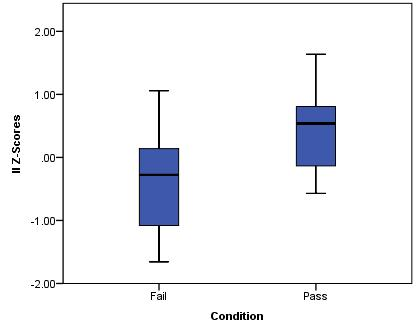
\includegraphics[ height=5cm]{II.jpg}
\caption{II Scores were significantly higher in the Pass condition $(p < 0.001)$, supporting \textbf{H1}.}\label{fig:II}
\end{figure}

\begin{table}[H]
\caption{Identifies Individuals (II) Items \label{II}}
\begin{center}
\begin{tabu}{|p{1.5cm} p{6cm}|}
\hline
\textbf{Survey Questions} &(On a scale of Strongly Disagree to Strongly Agree)\\
\hline
This robot: &
\begin{itemize}
\item Recognizes individual people
\item Remembers who people are
\item Cannot tell people apart
\item Figures out which people know each other
\end{itemize}\\
\hline
\end{tabu}
\end{center}
\end{table}

\subsubsection{Social Competence (SOC)}
A Kruskal-Wallis H Test was conducted to determine if there were differences in the SOC score between Genders. This scale was rated based on the robot appearing to have strong social skills. Distributions of the SOC scores between the Genders were not similar, as assessed by visual inspection. SOC scores for women (mean rank = 36.23) were statistically significantly higher than for men (mean rank = 26.68), \begin{math}\chi ^2= 4.311, p < .05 \end{math}.

%\begin{figure}[H]
%\centering
%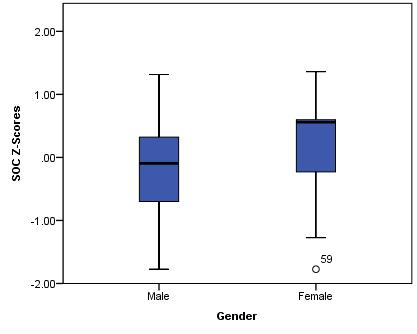
\includegraphics[ height=5cm]{SOC.jpg}
%\caption{SOC scores were significantly higher among female participants than males (p = 0.038). %}\label{fig:SOC}
%\end{figure}

\begin{table}[h]
\caption{Social Competence (SOC) Items}
\centering
\begin{tabu}{|p{1.5cm} p{6cm}|}
\hline
\textbf{Survey Questions} &(On a scale of Strongly Disagree to Strongly Agree)\\
\hline
This robot: &
\begin{itemize}
\item Is socially competent
\item Is socially aware
\item Is socially clueless
\item Has strong social skills
\end{itemize}\\
\hline
%\footnotetext{This item is reverse scored.}
\end{tabu}
\end{table}

%%%%%%%%%%%%%%%%%%%%%%%%%%%%%%%%%%%%%%%%%%%%%%%%%%%%%%%%%%%%%%%%%%%%%%%%%%%%%%%%
\section{Discussion}
\subsection{Summary of Findings}
Our study focused on how watching a robot successfully and unsuccessfully demonstrate a human-like social cognitive ability such as Theory of Mind influenced perception of cognitive and social intelligence and animacy. We intended to show that participants would rate the robot more favorably when it succeeded at the task when compared to the robot who failed the task. This held true for Perceived Intelligence and most of the scales from the PSI, but not for Animacy.

\subsection{Condition and Ratings of Intelligence and Animacy}
Our results show that watching a robot exhibit human-like cognitive capacities such as ToM influences whether they perceive the robot as intelligent as well as socially intelligent. Our data supported \textbf{H1}, as participants in the condition which watched the robot pass the task gave higher scores for Perceived Intelligence on the GQS than participants who watched the robot fail the task. The main effect for condition on Perceived Intelligence shows that participants had significant decrease in opinion of the robot after watching the video when the robot failed the task, and there was significant increase in how intelligent participants view the robot when it passed the task, supporting \textbf{H3} (Fig. \ref{fig:Intell-Before-After}). Regarding \textbf{H2}, we did not find significant differences in conditions for the Animacy GQS scale. 

\begin{figure}[h]
\centering
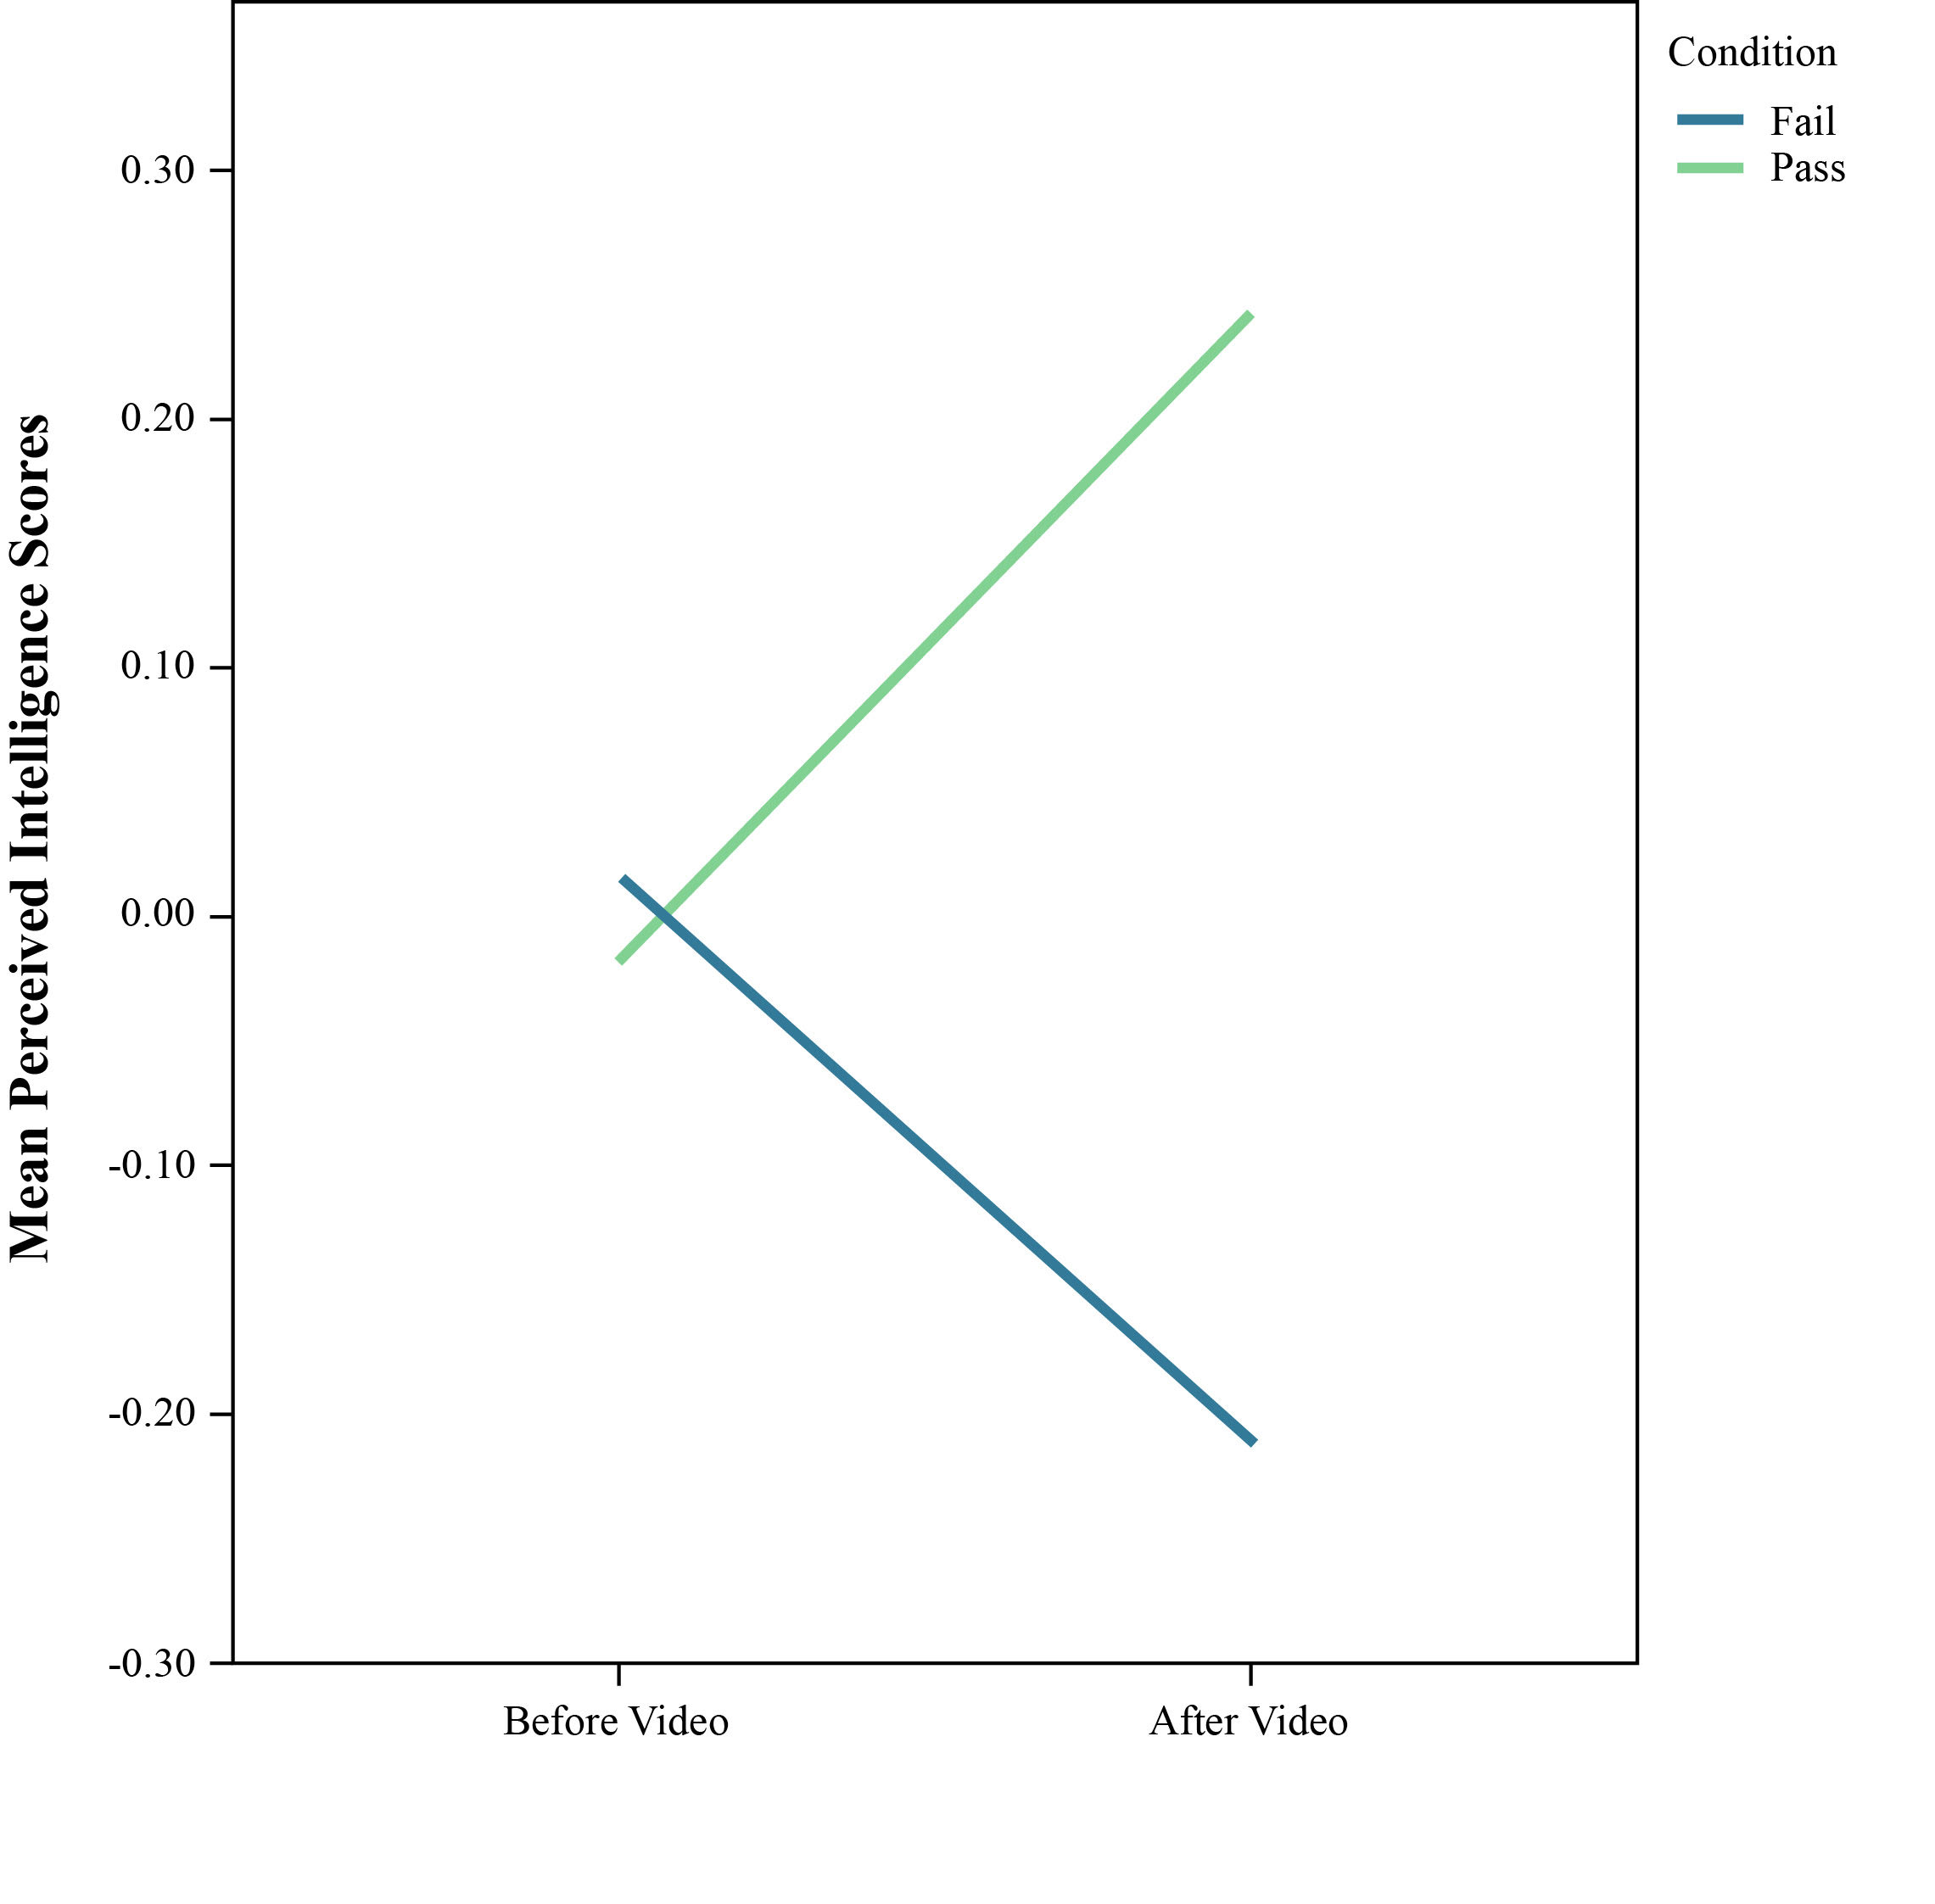
\includegraphics[height=6cm]{revised-before-after.jpg}
%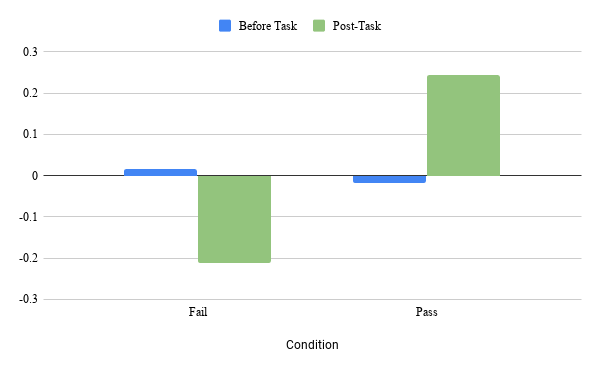
\includegraphics[height=5.5cm]{chart.png}
\caption{Mean GQS Perceived Intelligence Z-Scores by Condition before and after viewing the false-belief task\label{fig:Intell-Before-After}}
\end{figure}

\subsection{Condition and Perceived Social Intelligence}
Compared to participants in the \textbf{Fail} group, participants in the \textbf{Pass} condition scored higher on the robot's ability to recognize human cognition, predict human cognition, adapt to human cognition, predict human behavior, identify individuals, and social competence. This suggests that robots exhibiting Theory of Mind influence how much humans feel a robot is able to predict, adapt to, and detect human cognition and behavior. These results support \textbf{H1}, although the scales for recognizing human behavior and adapting to human behavior did not yield significant differences. 
\subsection{Participant Expectations}
Regarding \textbf{H4}, 45 out of 60 participants expected the robot to perform the task correctly. Furthermore, it appears when these expectations are met they view the robots as more intelligent than those who expected the robot to fail (Fig. \ref{fig:expectation}).

\begin{figure}[h]
\centering
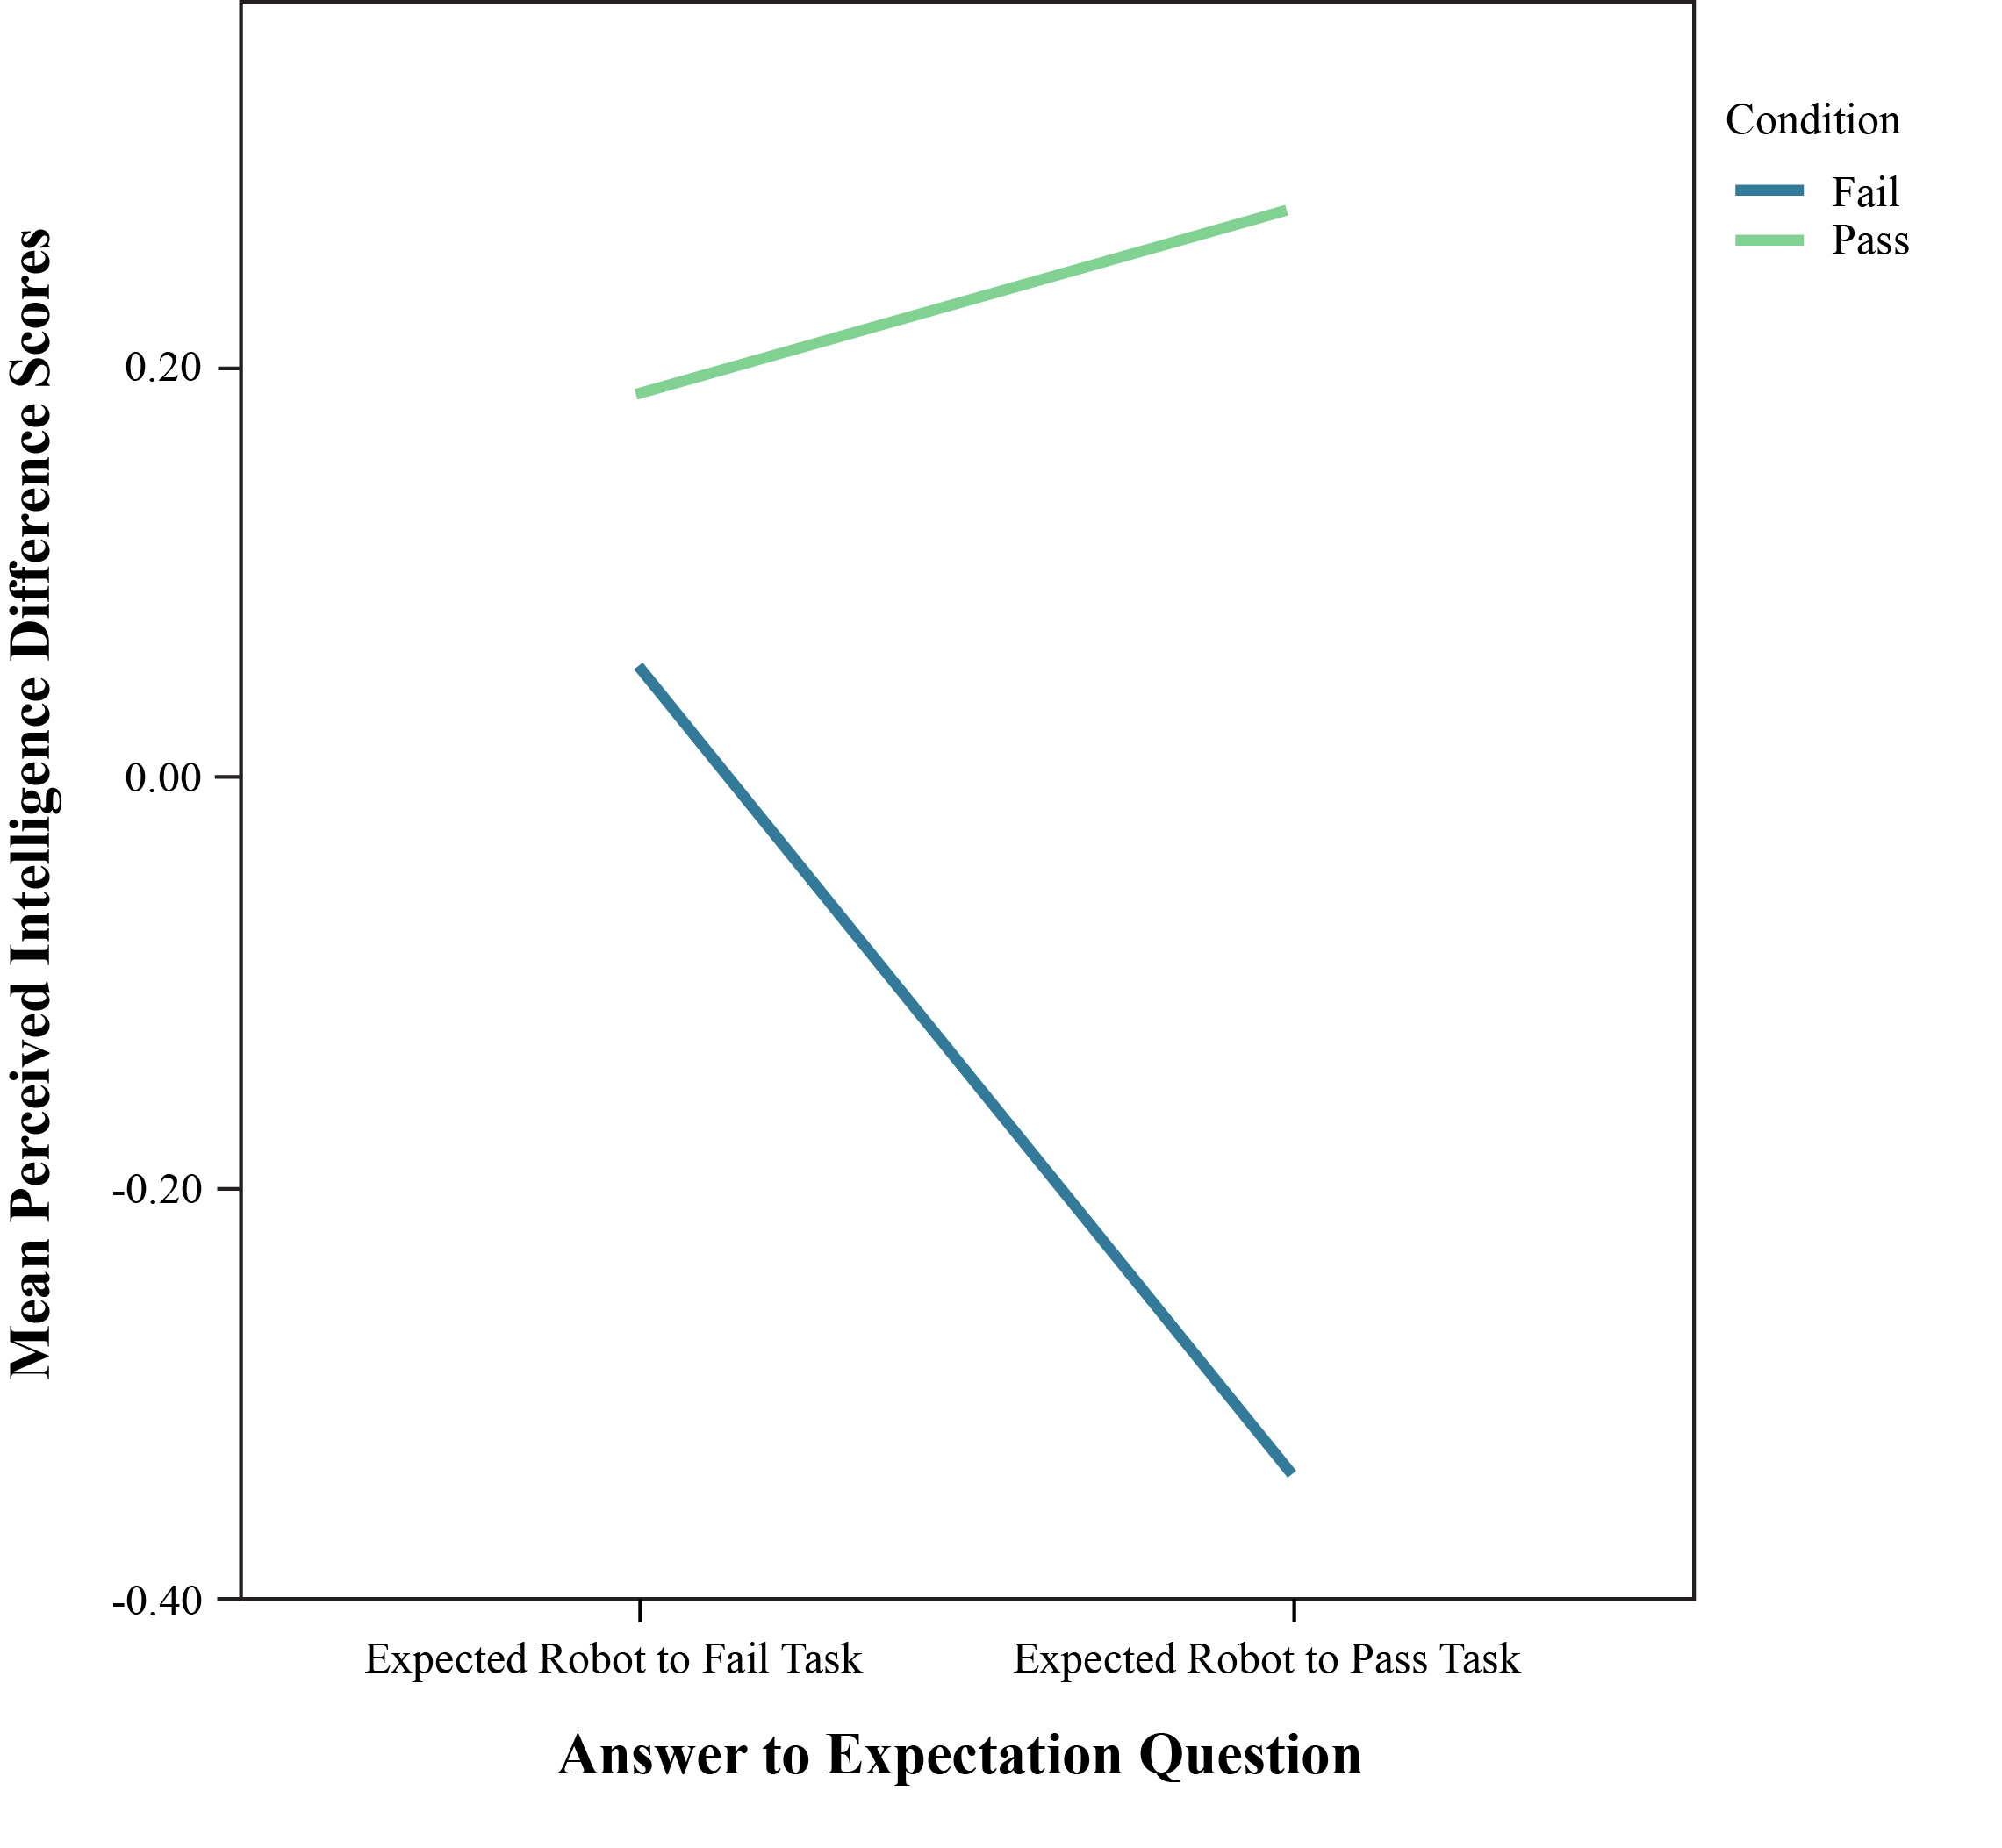
\includegraphics[ height=6cm]{revised-expectation.jpg}
\caption{Mean GQS Perceived Intelligence Z-Scores based on expectations and whether those expectations were met by participant condition\label{fig:expectation}}
\end{figure}

\subsection{Other Findings}
Although our experiment did not seek to examine the role of gender on perception we did find that Female participants scored the robot higher for PSI-SOC. Females seemed to see the robot as having stronger social skills than our Male participants. Our participant population was $60\%$ male. It is possible that with a larger female sample size this gender effect may disappear. 


%\begin{figure}[h!]
%\centering
%\includegraphics[ height=6.5cm]{Intell-Group.jpg}
%\caption{\label{fig:before-after}Mean scores for GQS Perceived Intelligence before and after watching the video}
%\end{figure}

%This study was designed with several dichotomous independent variables which made analysis challenging. Some statistical analysis isn't possible between multiple independent categorical variables. 

%Robots which interact and communicate with humans need to be able to process social information \cite{Dautenhahn}. Social intelligence is important in both social and non-social scenarios where robots are interacting with humans. 

\subsection{Limitations and Future Work}
%The sample size for this study was 60. A larger sample size could potentially yield a stronger effect size. A large portion of this population was also employed in fields related to science and information technology. A majority of participants had some degree of higher education (some college through PhD), with seven participants having only a high school diploma. 
This study has some limitations. The task in the video is staged and participants are not interacting directly with a robot. Embodiment is an aspect that could be incorporated into this study. Embodiment has been shown to have an impact on perception of robots \cite{MOLLAHOSSEINI201825}\cite{4813884}. More specifically, embodiment may play a key role in how humans perceive animacy. This study could be repeated with the robot performing the task in the same room as participants to investigate if there are any changes in animacy scores. Something to consider is also the age of participants. It could simply be that adults don't see a video of a robot as animate regardless of social competence. Future work could examine whether children give higher animacy scores than adults. Extensions for this experiment could also include a comparison of first-order and second-order ToM behavior. 

\subsection{Broader Implications}
Perception of cognitive and social capabilities in robots influences how humans interact with robots. When behavior defies social norms or displays social-cognitive deficits humans tend to be more critical.
%Our findings show that robots demonstrating human-like cognition increases perception of intelligence and social competence.
Our finding show that robots that do not demonstrate critical developmental concepts, such as Theory of Mind, are perceived as less socially intelligent than robots that do demonstrate such capacity.
These attitudes toward robots impact how likeable and beneficial people find their interactions with robots. People are more likely to continue using robots with which they have satisfying interactions. 
%Further study could yield results which could aid in robotics design.  

%Similar to the mock trial study referenced in the background section \cite{Maras2019} the robot in our study who failed the task was seen has less intelligent and was scored lower on all aspects of the Perceived Social Intelligence Survey.
 
%Implementing human-like cognitive processes is time and resource intensive. 


%\addtolength{\textheight}{-12cm}   
%%%%%%%%%%%%%%%%%%%%%%%%%%%%%%%%%%%%%%%%%%%%%%%%%%%%%%%%%%%%%%%%%%%%%%%%%%%%%%%%
%\section*{APPENDIX}


%\begin{table*}[ht]
%\caption{Questionnaire}
%\begin{tabular}{|c c c|}
%\hline
%\textbf{Survey Questions} &  \textbf{Source} &  \textbf{Scale} \\ %\hline
%\textbf{Before Task} &&\\ \hline 
%Please rate your impression of \textbf{robots in general} on these 5 %point scales.&&\\
%Incompetent/Competent &  GSQ &  Perceived Intelligence\\
%Ignorant/Knowledgeable &  GSQ &  Perceived Intelligence\\
%Irresponsible/Responsible &  GSQ &  Perceived Intelligence\\
%Unintelligent/Intelligent &  GSQ &  Perceived Intelligence\\
%Foolish/Sensible  &  GSQ &  Perceived Intelligence\\
%Dead/Alive &  GSQ &  Animacy \\
%Stagnant/Lively &  GSQ &  Animacy \\
%Mechanical/Organic &  GSQ &  Animacy \\
%Artificial/Lifelike &  GSQ &  Animacy \\
%Inert/Interactive &  GSQ &  Animacy \\
%Apathetic/Responsive &  GSQ &  Animacy \\ \hline

%\textbf{After Task} &&\\ \hline
%Incompetent/Competent &  GSQ &  Perceived Intelligence\\
%Ignorant/Knowledgeable &  GSQ &  Perceived Intelligence\\
%Irresponsible/Responsible &  GSQ &  Perceived Intelligence\\
%Unintelligent/Intelligent &  GSQ &  Perceived Intelligence\\
%Foolish/Sensible  &  GSQ &  Perceived Intelligence\\
%Dead/Alive &  GSQ &  Animacy \\
%Stagnant/Lively &  GSQ &  Animacy \\
%Mechanical/Organic &  GSQ &  Animacy \\
%Artificial/Lifelike &  GSQ &  Animacy \\
%Inert/Interactive &  GSQ &  Animacy \\
%Apathetic/Responsive &  GSQ &  Animacy \\ \hline

%On a scale of 1 to 5 (Strongly Disagree to Strongly Agree): &&\\
%This robot can figure out what people think & PSI & RC\\
%This robot knows when people are missing information & PSI & RC\\
%This robot can figure out what people can see & PSI & RC\\
%This robot understands others' perspectives & PSI & RC\\
%This robot anticipates others' beliefs & PSI & PC\\
%This robot figures out what people will believe in the future & PSI %& PC\\
%This robot knows ahead of time what people will think about certain %situations & PSI & PC\\
%This robot anticipates what people will think & PSI & PC\\
%
%This robot adapts its behavior based upon what people around it %know& PSI & AC\\
%This robot ignores what people are thinking *& PSI & AC\\
%This robot selects appropriate actions once it knows what others %think& PSI & AC\\
%This robot knows what to do when people are confused & PSI & AC\\%

%This robot anticipates people's behavior & PSI & PB\\
%This robot predicts human movements accurately & PSI & PB\\
%This robot has no idea what people are going to do & PSI & PB\\
%This robot knows how people will react to things it does & PSI & PB\\

%This robot recognizes individual people & PSI & II\\
%This robot remembers who people are & PSI & II\\
%This robot cannot tell people apart* & PSI & II\\
%This robot figures out which people know each other & PSI & II\\

%This robot is socially competent & PSI & SOC\\
%This robot is socially aware & PSI & SOC\\
%This robot is socially clueless* & PSI & SOC\\
%This robot has strong social skills & PSI & SOC\\ \hline
%
%\hline
%\end{tabular}
%\end{table*}

\section*{ACKNOWLEDGMENT}
This work was funded by the National Science Foundation (awards IIS-1757929 and IIS-1719027)
%%%%%%%%%%%%%%%%%%%%%%%%%%%%%%%%%%%%%%%%%%%%%%%%%%%%%%%%%%%%%%%%%%%%%%%%%%%%%%%%
\bibliographystyle{plain}
\bibliography{IEEEexample.bib}

\end{document}